\documentclass[tikz,border=8pt]{standalone}
\usepackage{amsmath}
\usetikzlibrary{arrows.meta,positioning}

\begin{document}
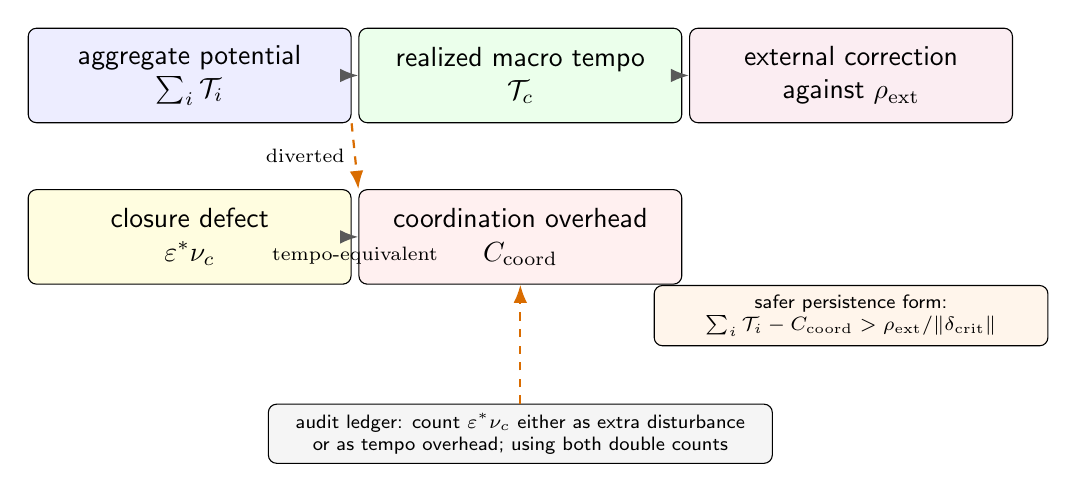
\begin{tikzpicture}[
  font=\sffamily,
  box/.style={draw, rounded corners=3pt, align=center, minimum width=41mm, minimum height=12mm, fill=white},
  note/.style={draw, rounded corners=3pt, align=center, font=\sffamily\scriptsize, fill=white},
  arrow/.style={-Latex, thick, draw=black!65},
  warn/.style={-Latex, thick, dashed, draw=orange!85!black}
]

\node[box, fill=blue!7] (sum) at (-4.2,1.2)
  {aggregate potential\\$\sum_i \mathcal T_i$};
\node[box, fill=green!8] (macro) at (0,1.2)
  {realized macro tempo\\$\mathcal T_c$};
\node[box, fill=red!6] (coord) at (0,-0.85)
  {coordination overhead\\$C_{\rm coord}$};
\node[box, fill=purple!7] (external) at (4.2,1.2)
  {external correction\\against $\rho_{\rm ext}$};
\node[box, fill=yellow!12] (closure) at (-4.2,-0.85)
  {closure defect\\$\varepsilon^\ast \nu_c$};

\draw[arrow] (sum.east) -- (macro.west);
\draw[arrow] (macro.east) -- (external.west);
\draw[arrow] (closure.east) -- node[below, font=\scriptsize] {tempo-equivalent} (coord.west);
\draw[warn] (sum.south east) -- node[left, font=\scriptsize] {diverted} (coord.north west);

\node[note, fill=gray!8, minimum width=64mm] (ledger) at (0,-3.35)
  {audit ledger: count $\varepsilon^\ast\nu_c$ either as extra disturbance\\or as tempo overhead; using both double counts};
\draw[warn] (ledger.north) -- (coord.south);

\node[note, fill=orange!8, minimum width=50mm] at (4.2,-1.85)
  {safer persistence form:\\$\sum_i\mathcal T_i - C_{\rm coord} > \rho_{\rm ext}/\lVert\delta_{\rm crit}\rVert$};

\end{tikzpicture}
\end{document}
